% Provenance (never printed): cycle 4 SVT, "La planete Terre": earthquakes,
% faults, seismic waves and their recording, magnitude and intensity, the
% link with plate boundaries; natural hazards (tsunamis) and prevention; see
% sources/book1/PROVENANCE.md. Book 1, grade 7, chapter 3.
% Vocabulary guard: P and S waves are named in prose only (they were named in
% g6.4, defined in Book 2 g11); "sediment" not before g7.4; "intensity" is
% always the earthquake's (homograph with physics: linker STOP list).
\chapter{Los terremotos}\label{ch:g7:earthquakes}

En la mañana del 26~de diciembre de 2004, bajo el \omterm{def:g2:water-on-earth:ocean}{mar}, frente al extremo
noroeste de Sumatra, en Indonesia, las \omterm{def:g3:stones-pebbles-sand:rock}{rocas} se rompieron a lo largo de una
\omterm{def:g7:earthquakes:fault}{falla}: fue uno de los mayores \omterm{def:g4:volcanoes-earthquakes-first-look:earthquake}{terremotos} jamás medidos. En la \omterm{def:g1:landscapes-around-us:water}{costa} cercana
de Sumatra, el \omterm{def:g2:water-on-earth:ocean}{mar} se elevó en olas de hasta \qty{51}{m} de altura, que
penetraron hasta \qty{5}{km} tierra adentro. En las horas siguientes, las
olas cruzaron el \omterm{def:g2:water-on-earth:ocean}{océano} Índico y golpearon las \omterm{def:g1:landscapes-around-us:water}{costas} de quince países,
hasta en África. Murieron unas 230\,000 personas. En aquella época no
había ningún sistema de alerta en el \omterm{def:g2:water-on-earth:ocean}{océano} Índico.
% ledger: usgs:largest, nws:tsunami-2004

\begin{omfigure}
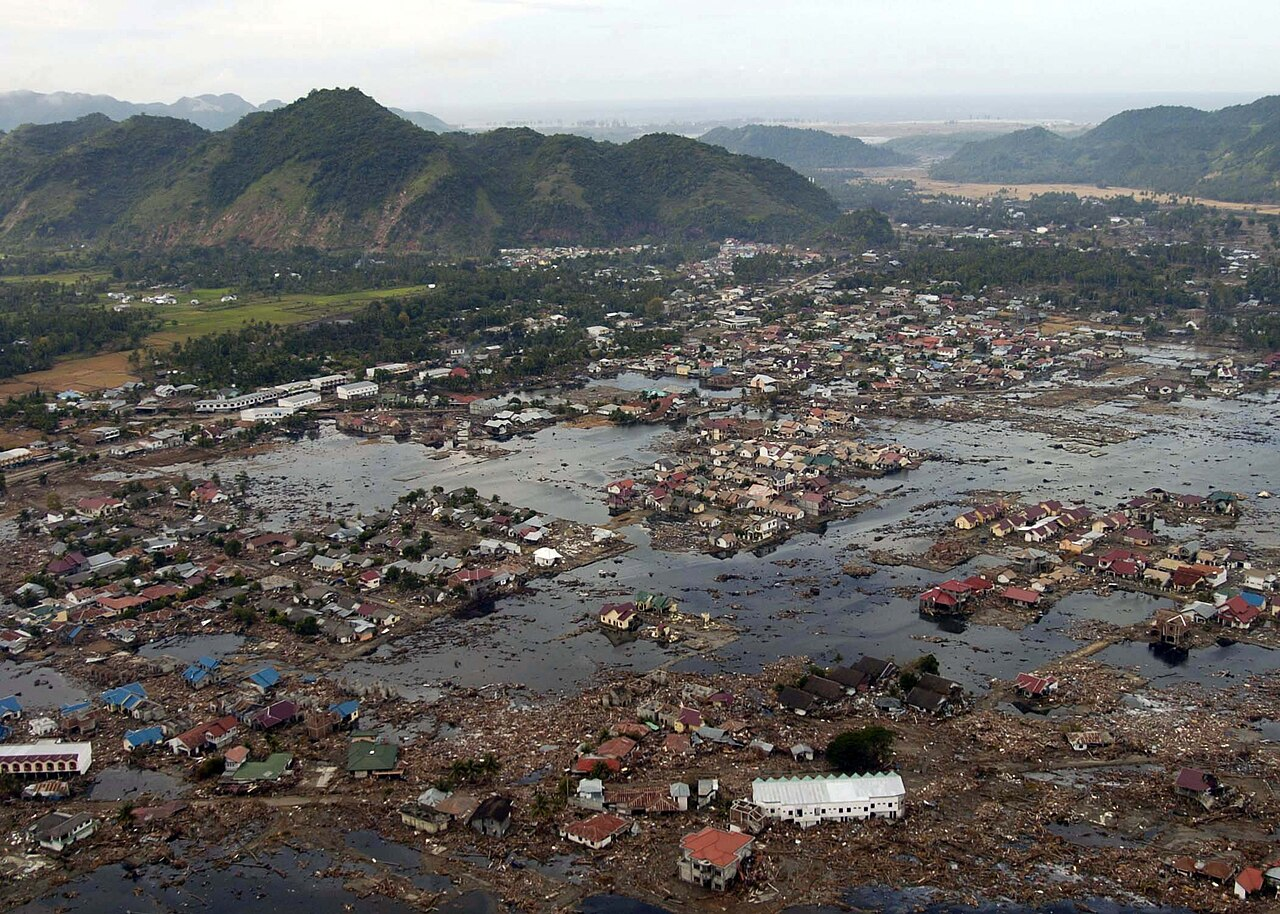
\includegraphics[width=0.78\linewidth]{images/book1/g7-tsunami-village.jpg}

{\small Un pueblo cercano a la \omterm{def:g1:landscapes-around-us:water}{costa} de Sumatra una semana después del
\omterm{def:g7:earthquakes:tsunami}{tsunami} del 26~de diciembre de 2004. Fotografía de la U.S. Navy, por
Philip~A. McDaniel (dominio público, vía Wikimedia Commons).}
% ledger: commons:tsunami-village
\label{fig:g7:earthquakes:tsunami-village}
\end{omfigure}

¿Cómo se rompen las \omterm{def:g3:stones-pebbles-sand:rock}{rocas}? ¿Cómo averiguan los científicos, en pocos
minutos, dónde se produjo un \omterm{def:g4:volcanoes-earthquakes-first-look:earthquake}{terremoto} y cómo fue de grande? ¿Y por qué, horas
después, se elevó el \omterm{def:g2:water-on-earth:ocean}{mar} en \omterm{def:g1:landscapes-around-us:water}{costas} donde nadie había sentido nada?

\begin{recall}
Un \emph{\omterm{def:g4:volcanoes-earthquakes-first-look:earthquake}{terremoto}} es una sacudida brusca del suelo causada por \omterm{def:g3:stones-pebbles-sand:rock}{rocas} que
se rompen y se deslizan en las profundidades
(\cref{ch:g4:volcanoes-earthquakes-first-look}). La envoltura exterior de
la Tierra está hecha de \omterm{def:g7:plate-tectonics:plate}{placas}, y el 92~\% de los grandes \omterm{def:g4:volcanoes-earthquakes-first-look:earthquake}{terremotos} se
producen a menos de \qty{300}{km} de un \omterm{def:g7:plate-tectonics:plate-boundary}{límite de placas}
(\cref{ch:g7:plate-tectonics}). Cuando se produce un \omterm{def:g4:volcanoes-earthquakes-first-look:earthquake}{terremoto}, unas ondas
recorren las \omterm{def:g3:stones-pebbles-sand:rock}{rocas} de toda la Tierra: unas más rápidas (las ondas~P) y
otras más lentas (las ondas~S); midiendo el tiempo que tardan, los
científicos descubrieron el \omterm{def:g6:inside-the-earth:layers}{núcleo} (\cref{ch:g6:inside-the-earth}).
\end{recall}

\section{Rocas que se rompen}

Las \omterm{def:g7:plate-tectonics:plate}{placas} se mueven unos pocos centímetros al año, pero sus bordes son
ásperos: se quedan enganchados mientras el resto de las \omterm{def:g7:plate-tectonics:plate}{placas} sigue
moviéndose. Las \omterm{def:g3:stones-pebbles-sand:rock}{rocas} cercanas al borde se doblan un poco, como una regla
que empujas por los dos extremos, y van acumulando energía. Cuando el empuje
vence por fin al rozamiento, las \omterm{def:g3:stones-pebbles-sand:rock}{rocas} se desenganchan de golpe y se
deslizan: ese deslizamiento brusco es el \omterm{def:g4:volcanoes-earthquakes-first-look:earthquake}{terremoto}.
% ledger: usgs:eq-basics

\begin{definition}[Falla]\label{def:g7:earthquakes:fault}
Una \emph{falla}\index{falla} es una rotura de las \omterm{def:g3:stones-pebbles-sand:rock}{rocas} a lo largo de la
cual los dos bloques situados a cada lado se han desplazado uno respecto
al otro. Durante un \omterm{def:g4:volcanoes-earthquakes-first-look:earthquake}{terremoto}, los bloques se deslizan bruscamente a lo
largo de la falla; cuanto mayores son la falla y el deslizamiento, mayor es
el \omterm{def:g4:volcanoes-earthquakes-first-look:earthquake}{terremoto}.
\end{definition}

Un \omterm{def:g7:plate-tectonics:plate-boundary}{límite de placas} está formado por muchas \omterm{def:g7:earthquakes:fault}{fallas}, y la mayoría de los
\omterm{def:g4:volcanoes-earthquakes-first-look:earthquake}{terremotos} del mundo se producen en ellas. Pero también hay \omterm{def:g7:earthquakes:fault}{fallas} en el
interior de las \omterm{def:g7:plate-tectonics:plate}{placas}, y algunas de ellas también pueden romperse. Cuando
una \omterm{def:g7:earthquakes:fault}{falla} grande se rompe cerca de la superficie, el deslizamiento se ve en
el suelo: un escalón en un campo, una carretera cortada en dos, una valla
o una hilera de árboles desplazadas hacia un lado.
% ledger: usgs:eq-basics

\begin{omfigure}
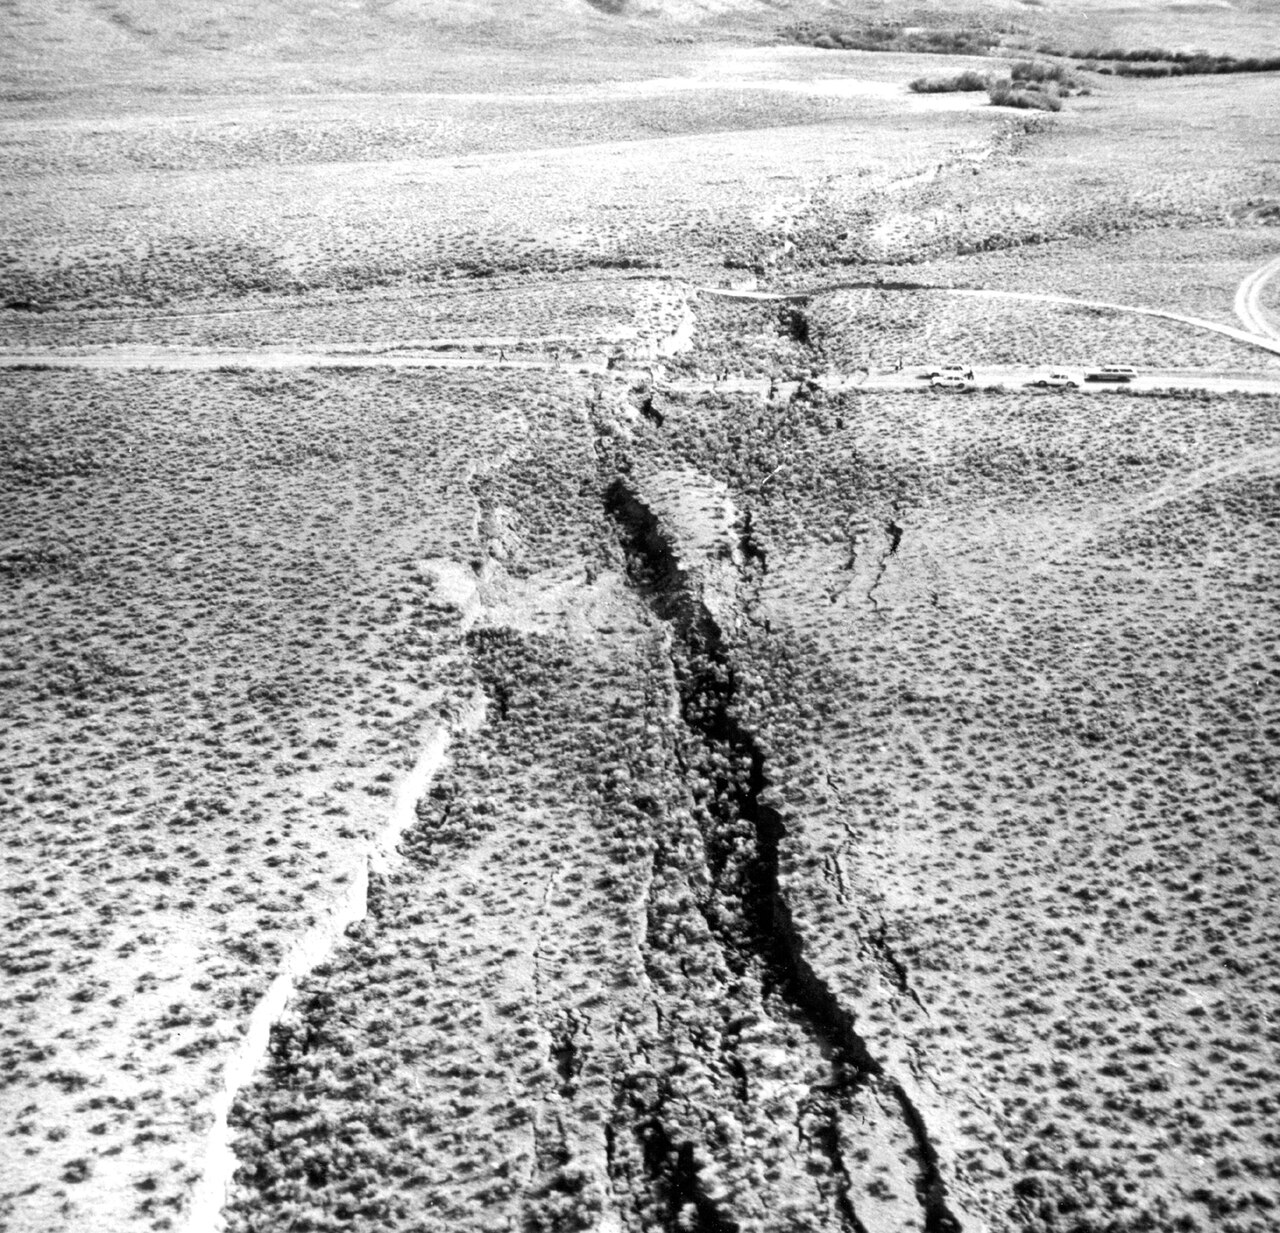
\includegraphics[width=0.62\linewidth]{images/book1/g7-borah-scarp.jpg}

{\small Escalones en el suelo dejados por el \omterm{def:g4:volcanoes-earthquakes-first-look:earthquake}{terremoto} de Borah Peak de
1983, en Idaho (Estados Unidos), vistos desde el aire: a lo largo de la
\omterm{def:g7:earthquakes:fault}{falla}, un lado se hundió respecto al otro, y el escalón cruza la carretera
en la parte de arriba. Fotografía: R.~E. Wallace, U.S. Geological Survey
(dominio público, vía Wikimedia Commons).}
% ledger: commons:borah-scarp
\label{fig:g7:earthquakes:borah}
\end{omfigure}

\begin{definition}[Hipocentro y epicentro]\label{def:g7:earthquakes:focus}
El \emph{hipocentro}\index{hipocentro} (o foco) de un \omterm{def:g4:volcanoes-earthquakes-first-look:earthquake}{terremoto} es el lugar
del subsuelo, en la \omterm{def:g7:earthquakes:fault}{falla}, donde empieza el deslizamiento. El
\emph{epicentro}\index{epicentro} es el punto de la superficie de la Tierra
situado justo encima del hipocentro.
\end{definition}

El \omterm{def:g7:earthquakes:focus}{hipocentro} suele estar a una profundidad de unos pocos kilómetros a unas
pocas decenas de kilómetros. De los 7\,031 \omterm{def:g4:volcanoes-earthquakes-first-look:earthquake}{terremotos} de \omterm{def:g7:earthquakes:magnitude}{magnitud}~6 o más
registrados entre 1976 y 2025, 5\,561 --- el 79~\% --- tuvieron su
\omterm{def:g7:earthquakes:focus}{hipocentro} a menos de \qty{70}{km} de profundidad. Pero 483 empezaron a
más de \qty{300}{km}, y el más profundo a \qty{688}{km}: estos \omterm{def:g4:volcanoes-earthquakes-first-look:earthquake}{terremotos}
profundos se producen donde una \omterm{def:g7:plate-tectonics:plate}{placa} se hunde bajo otra, dentro de la
\omterm{def:g7:plate-tectonics:plate}{placa} que se hunde.
% ledger: data:usgs-comcat (figdata/grade-7/quake_counts.py, part depth)

Un gran \omterm{def:g4:volcanoes-earthquakes-first-look:earthquake}{terremoto} rara vez llega solo. A menudo le siguen otros más
pequeños en el mismo lugar, las \emph{réplicas}, durante semanas, meses e
incluso años. A veces lo preceden \omterm{def:g4:volcanoes-earthquakes-first-look:earthquake}{terremotos} más pequeños, pero nadie
puede saber que eran avisos hasta que se ha producido el grande: los
científicos no pueden predecir los \omterm{def:g4:volcanoes-earthquakes-first-look:earthquake}{terremotos}. Solo pueden decir qué
\omterm{def:g7:earthquakes:fault}{fallas} volverán a romperse algún día y ayudar a la gente a prepararse.
% ledger: usgs:eq-basics, usgs:seismograph

\begin{omfigure}
\begin{tikzpicture}[font=\small, x=1cm, y=1cm]
  % a block of crust seen in perspective: front face and top face
  \def\dx{2.2}\def\dy{1.3}
  % top surface: two blocks separated by the fault trace
  \fill[green!12] (0,0) -- (4.6,0) -- (4.6+\dx,\dy) -- (\dx,\dy) -- cycle;
  \fill[green!18] (4.6,0) -- (9,0) -- (9+\dx,\dy) -- (4.6+\dx,\dy) -- cycle;
  % front face
  \fill[brown!30] (0,0) -- (4.6,0) -- (3.4,-4) -- (0,-4) -- cycle;
  \fill[brown!40] (4.6,0) -- (9,0) -- (9,-4) -- (3.4,-4) -- cycle;
  % right face
  \fill[brown!22] (9,0) -- (9+\dx,\dy) -- (9+\dx,\dy-4) -- (9,-4) -- cycle;
  % fault plane on the front face and trace on top
  \draw[very thick, red!70!black] (4.6,0) -- (3.4,-4);
  \draw[very thick, red!70!black] (4.6,0) -- (4.6+\dx,\dy);
  % slip arrows
  \draw[-{Stealth[length=2.5mm]}, thick] (2.6,-0.35) -- (1.6,-0.35);
  \draw[-{Stealth[length=2.5mm]}, thick] (6.4,-0.35) -- (7.4,-0.35);
  \node[font=\footnotesize, anchor=south] at (2.1,-0.3) {bloque 1};
  \node[font=\footnotesize, anchor=south] at (6.9,-0.3) {bloque 2};
  % focus and waves
  \coordinate (F) at (3.95,-2.4);
  \foreach \r in {0.5,1.0,1.5,2.0}
    \draw[blue!60, dashed] (F) circle (\r);
  \fill[red!80!black] (F) circle (0.13);
  % epicentre: on the surface, straight above the focus (front edge of the top face)
  \coordinate (E) at (3.95,0);
  \draw[black!60, densely dotted, thick] (F) -- (E);
  \node[star, star points=5, star point ratio=2.4, fill=orange, draw=black, inner sep=1.4pt] at (E) {};
  % labels
  \node[anchor=west] at (9.5,-2.3) {hipocentro};
  \draw[black!60] (9.45,-2.3) -- (4.1,-2.4);
  \node[anchor=south west] at (4.9,1.9) {epicentro};
  \draw[black!60] (4.95,1.95) -- (4.05,0.12);
  \node[anchor=south, red!70!black] at (6.8,1.3) {falla};
  \node[anchor=east, blue!60!black, align=right] at (-0.15,-2.6) {las ondas se propagan\\en todas direcciones};
  \draw[blue!60, -{Stealth}] (-0.1,-2.6) -- (1.9,-2.5);
\end{tikzpicture}

{\small Una \omterm{def:g7:earthquakes:fault}{falla}, el \omterm{def:g7:earthquakes:focus}{hipocentro} y el \omterm{def:g7:earthquakes:focus}{epicentro} (un dibujo, no a escala).
Los dos bloques se deslizan uno junto a otro a lo largo de la \omterm{def:g7:earthquakes:fault}{falla} (en
rojo); el deslizamiento empieza en el \omterm{def:g7:earthquakes:focus}{hipocentro}, y desde él se propagan
ondas en todas direcciones, como las ondas en un estanque. El \omterm{def:g7:earthquakes:focus}{epicentro}
(estrella) está en la superficie, justo encima del \omterm{def:g7:earthquakes:focus}{hipocentro}.}
% ledger: usgs:eq-basics
\label{fig:g7:earthquakes:fault}
\end{omfigure}


\section{Registrar un terremoto}

\begin{definition}[Sismómetro y sismograma]\label{def:g7:earthquakes:seismometer}
Un \emph{sismómetro}\index{sismometro@sismómetro} es un instrumento que
registra las sacudidas del suelo. Su registro, una línea ondulada trazada
en función del tiempo, es un \emph{sismograma}\index{sismograma}.
\end{definition}

La idea de un \omterm{def:g7:earthquakes:seismometer}{sismómetro} es sencilla. Un bastidor está bien sujeto al
suelo; de él cuelga una masa pesada, sostenida por un muelle. Cuando el
suelo tiembla, el bastidor tiembla con él, pero la masa pesada, sostenida
solo por su muelle, se queda casi quieta. El instrumento registra el
movimiento del bastidor respecto a la masa inmóvil: es el movimiento del
suelo. En el dibujo de abajo, una plumilla sujeta a la masa lo traza sobre
un papel enrollado en un tambor que gira.
% ledger: usgs:seismograph

\begin{omfigure}
\begin{tikzpicture}[font=\small, x=1cm, y=1cm]
  \begin{scope}
    % ground
    \fill[brown!30] (-0.6,-0.6) rectangle (5.0,0);
    \draw[decorate, decoration={snake, amplitude=1.2pt, segment length=6pt}, brown!70!black, thick]
      (-0.6,0) -- (5.0,0);
    % frame
    \fill[black!55] (0,0) rectangle (0.25,3.2);
    \fill[black!55] (0,3.0) rectangle (2.4,3.25);
    % spring and weight
    \draw[decorate, decoration={coil, aspect=0.5, segment length=3pt, amplitude=4pt}, thick]
      (2.1,3.0) -- (2.1,2.1);
    \fill[black!80] (1.7,1.45) rectangle (2.5,2.1);
    \node[white, font=\scriptsize] at (2.1,1.78) {masa};
    % pen arm and drum
    \draw[thick] (2.5,1.75) -- (3.45,1.75);
    \fill (3.45,1.75) circle (0.05);
    \draw[thick, fill=white] (3.95,1.75) circle (0.5);
    \draw[thick] (3.95,1.25) -- (3.95,0);
    \draw[-{Stealth}, black!60] (4.55,2.2) arc (40:-40:0.7);
    % labels
    \node[anchor=east, align=right, font=\footnotesize] at (-0.1,2.3) {bastidor sujeto\\al suelo};
    \node[anchor=west, font=\footnotesize] at (2.6,2.65) {muelle};
    \draw[black!60] (2.55,2.65) -- (2.25,2.6);
    \node[anchor=north, align=center, font=\footnotesize] at (2.1,1.35) {masa pesada:\\se queda quieta};
    \node[anchor=west, align=left, font=\footnotesize] at (4.7,1.05) {tambor que gira\\con papel};
    \node[anchor=north, font=\footnotesize] at (2.2,-0.65) {el suelo tiembla};
  \end{scope}
  \begin{scope}[xshift=7.2cm, yshift=0.4cm]
    \begin{axis}[width=7.6cm, height=4.2cm, xmin=0, xmax=60, ymin=-1.1, ymax=1.1,
        axis x line=bottom, axis y line=none, xlabel={tiempo (segundos)},
        tick label style={font=\scriptsize}, label style={font=\footnotesize}, clip=false]
      \addplot[black, line width=0.4pt] table[x=t, y=v] {figdata/out/grade-7-epicentre-m-trace.dat};
      \draw[blue!70!black, -{Stealth[length=2mm]}] (axis cs:10,1.45) -- (axis cs:10,0.45);
      \node[blue!70!black, font=\scriptsize, anchor=south east] at (axis cs:10.5,1.45) {llegan las ondas más rápidas};
      \draw[red!70!black, -{Stealth[length=2mm]}] (axis cs:20,1.45) -- (axis cs:20,1.05);
      \node[red!70!black, font=\scriptsize, anchor=south west] at (axis cs:19.5,1.45) {llegan las ondas más lentas};
      \draw[{Stealth[length=2mm]}-{Stealth[length=2mm]}] (axis cs:10,-0.75) -- (axis cs:20,-0.75);
      \node[font=\scriptsize, anchor=east] at (axis cs:9,-0.75) {retraso: 10 s};
    \end{axis}
  \end{scope}
\end{tikzpicture}

{\small A la izquierda: el principio de un \omterm{def:g7:earthquakes:seismometer}{sismómetro} (un dibujo). A la
derecha: un \omterm{def:g7:earthquakes:seismometer}{sismograma} trazado para este libro (no es un registro real): la
línea está tranquila, después llegan las ondas más rápidas y, diez segundos
más tarde, las más lentas y más grandes.}
% ledger: usgs:seismograph (trace drawn by figdata/grade-7/epicentre.py, part m-trace)
\label{fig:g7:earthquakes:seismometer}
\end{omfigure}

\subsection*{¿A qué distancia se produjo el terremoto?}

Un \omterm{def:g7:earthquakes:seismometer}{sismograma} dice algo más que ``el suelo ha temblado''. Las ondas más
rápidas llegan siempre primero, y las más lentas después. Cerca del
\omterm{def:g7:earthquakes:focus}{hipocentro} llegan casi a la vez; lejos, las ondas lentas se van quedando
cada vez más atrás, igual que, durante una \omterm{def:g5:natural-hazards:storm}{tormenta}, el trueno llega cada
vez más tarde tras el relámpago cuando la \omterm{def:g5:natural-hazards:storm}{tormenta} está lejos. Así que el
retraso entre las dos llegadas indica la distancia al \omterm{def:g4:volcanoes-earthquakes-first-look:earthquake}{terremoto}.
% ledger: usgs:seismograph

¿Cuántos kilómetros por cada segundo de retraso? Depende de las
velocidades de las dos ondas en las \omterm{def:g3:stones-pebbles-sand:rock}{rocas} que atraviesan. Con las
velocidades del modelo de referencia de la Tierra
(\cref{ch:g6:inside-the-earth}), cada segundo de retraso equivale a unos
\qty{7}{km} en la \omterm{def:g6:inside-the-earth:layers}{corteza} superior y a \qty{9}{km} en la \omterm{def:g6:inside-the-earth:layers}{corteza} inferior.
En los ejercicios de este capítulo usamos el valor redondo de \qty{8}{km}
por cada segundo.
% ledger: data:prem (computed in figdata/grade-7/epicentre.py, part rule)

\begin{method}[Hallar el epicentro con tres estaciones]\label{met:g7:earthquakes:three-circles}
\begin{enumerate}
  \item En el \omterm{def:g7:earthquakes:seismometer}{sismograma} de cada estación, lee el retraso entre la llegada
        de las ondas más rápidas y la de las más lentas.
  \item Convierte cada retraso en una distancia (aquí: $8 \times$ el
        retraso en segundos, en kilómetros).
  \item En un \omterm{def:g2:drawing-to-map:map}{mapa}, traza alrededor de cada estación un círculo cuyo radio
        sea su distancia. El \omterm{def:g7:earthquakes:focus}{epicentro} está en algún punto de cada círculo.
  \item Con dos círculos suele haber dos puntos posibles; el tercer círculo
        solo pasa por uno de ellos: ese es el \omterm{def:g7:earthquakes:focus}{epicentro}.
\end{enumerate}
\end{method}

\begin{example}[Tres círculos]\label{ex:g7:earthquakes:three-circles}
Tres estaciones registran el mismo \omterm{def:g4:volcanoes-earthquakes-first-look:earthquake}{terremoto}. Los retrasos son de
\qty{10}{s} en la estación~M1, \qty{11.25}{s} en M2 y \qty{9.75}{s} en M3.
Las distancias son $8 \times 10 = \qty{80}{km}$,
$8 \times 11.25 = \qty{90}{km}$ y $8 \times 9.75 = \qty{78}{km}$. Los tres
círculos, trazados abajo, se cortan en un único punto: el \omterm{def:g7:earthquakes:focus}{epicentro}.
% ledger: usgs:seismograph (figdata/grade-7/epicentre.py, parts m-stations and m-circles)
\end{example}

\begin{omfigure}
\begin{tikzpicture}
  \begin{axis}[axis equal image, width=8.2cm, xmin=-150, xmax=170, ymin=-160, ymax=160,
      xtick={-120,-80,...,160}, ytick={-120,-80,...,120}, grid=both, grid style={black!12},
      tick label style={font=\scriptsize}, xlabel={km}, ylabel={km}, label style={font=\footnotesize}]
    \addplot[blue!60!black, line width=0.6pt] table[x=x, y=y] {figdata/out/grade-7-epicentre-m-circles.dat};
    \addplot[only marks, mark=triangle*, mark size=3pt, black,
        nodes near coords, point meta=explicit symbolic,
        nodes near coords style={font=\scriptsize, anchor=north, yshift=-2pt}]
      table[x=x, y=y, meta=name] {figdata/out/grade-7-epicentre-m-stations.dat};
    \node[star, star points=5, star point ratio=2.4, fill=orange, draw=black, inner sep=1.6pt] at (axis cs:0,0) {};
    \draw[black!60] (axis cs:-4,-4) -- (axis cs:-60,-75);
    \node[font=\scriptsize, anchor=north east, inner sep=1pt] at (axis cs:-60,-75) {epicentro};
  \end{axis}
\end{tikzpicture}

{\small Cada círculo está centrado en una estación (triángulo), con un
radio igual a la distancia entre esa estación y el \omterm{def:g4:volcanoes-earthquakes-first-look:earthquake}{terremoto}. Los tres
círculos se cortan en un solo punto, el \omterm{def:g7:earthquakes:focus}{epicentro} (estrella).}
% ledger: usgs:seismograph (figdata/grade-7/epicentre.py, parts m-stations and m-circles)
\label{fig:g7:earthquakes:three-circles}
\end{omfigure}

\begin{omfigure}
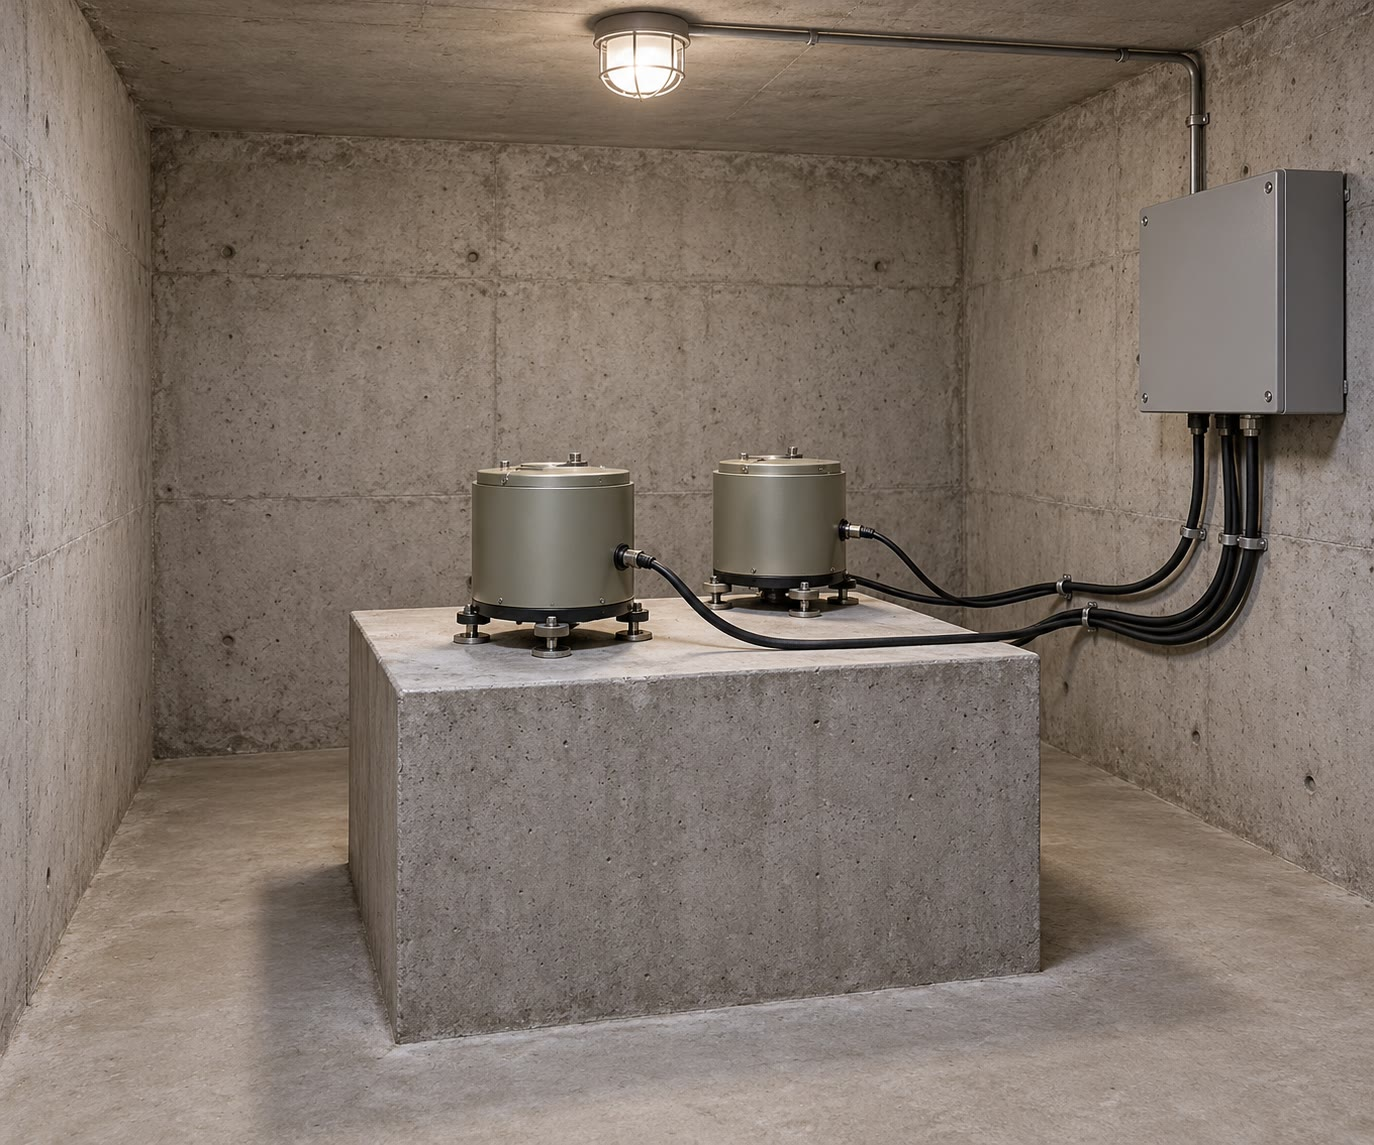
\includegraphics[width=0.58\linewidth]{images/book1/ai/g7-seismometer-vault.jpg}

{\small \omterm{def:g7:earthquakes:seismometer}{Sismómetros} en una sala subterránea silenciosa, colocados sobre un
pilar de hormigón apoyado en la \omterm{def:g3:stones-pebbles-sand:rock}{roca}, lejos de las carreteras y de las
máquinas (ilustración generada por IA de una escena genérica).}
\label{fig:g7:earthquakes:vault}
\end{omfigure}

\section{¿Cómo de grande? Magnitud e intensidad}

Dos números distintos describen un \omterm{def:g4:volcanoes-earthquakes-first-look:earthquake}{terremoto}, y a menudo se confunden.

\begin{definition}[Magnitud]\label{def:g7:earthquakes:magnitude}
La \emph{magnitud}\index{magnitud} de un \omterm{def:g4:volcanoes-earthquakes-first-look:earthquake}{terremoto} mide su tamaño: la
energía liberada en su origen. Se calcula a partir de los \omterm{def:g7:earthquakes:seismometer}{sismogramas}.
Cada \omterm{def:g4:volcanoes-earthquakes-first-look:earthquake}{terremoto} tiene una sola magnitud, escrita con un decimal, como 6.3
o 9.1.
\end{definition}

\begin{definition}[Intensidad]\label{def:g7:earthquakes:intensity}
La \emph{intensidad}\index{intensidad} de un \omterm{def:g4:volcanoes-earthquakes-first-look:earthquake}{terremoto} en un lugar
describe con qué fuerza tembló allí el suelo, a partir de lo que sintió la
gente y de los daños que vio. Se escribe en números romanos, de I (no se
siente) a XII (destrucción total). Un mismo \omterm{def:g4:volcanoes-earthquakes-first-look:earthquake}{terremoto} tiene muchas
intensidades: una distinta en cada lugar.
\end{definition}

La escala de magnitudes sube deprisa. Cada paso de 1 en la \omterm{def:g7:earthquakes:magnitude}{magnitud}
significa ondas unas 10~veces más grandes en el \omterm{def:g7:earthquakes:seismometer}{sismograma} y unas 32~veces
más energía liberada. Un \omterm{def:g4:volcanoes-earthquakes-first-look:earthquake}{terremoto} de \omterm{def:g7:earthquakes:magnitude}{magnitud}~8 libera unas
$32 \times 32 \approx 1000$ veces más energía que uno de \omterm{def:g7:earthquakes:magnitude}{magnitud}~6.
% ledger: usgs:mag-energy

\begin{method}[Comparar dos magnitudes]\label{met:g7:earthquakes:magnitudes}
Para comparar la energía de dos \omterm{def:g4:volcanoes-earthquakes-first-look:earthquake}{terremotos}, cuenta los pasos enteros que
hay entre sus \omterm{def:g7:earthquakes:magnitude}{magnitudes} y multiplica por 32 una vez por cada paso:
1~paso, 32~veces; 2~pasos, unas 1000~veces; 3~pasos, unas 32\,000~veces.
\end{method}

\begin{example}[Magnitud 9 y magnitud 7]\label{ex:g7:earthquakes:nine-seven}
El \omterm{def:g4:volcanoes-earthquakes-first-look:earthquake}{terremoto} de 2004 frente a Sumatra tuvo una \omterm{def:g7:earthquakes:magnitude}{magnitud} de 9.1. Un
\omterm{def:g4:volcanoes-earthquakes-first-look:earthquake}{terremoto} de \omterm{def:g7:earthquakes:magnitude}{magnitud}~7.1 está dos pasos por debajo: liberó
$32 \times 32 = 1024$, es decir, unas 1000~veces menos energía.
% ledger: usgs:largest, usgs:mag-energy
\end{example}

Los mayores \omterm{def:g4:volcanoes-earthquakes-first-look:earthquake}{terremotos} jamás medidos se produjeron todos donde una \omterm{def:g7:plate-tectonics:plate}{placa}
se hunde bajo otra: \omterm{def:g7:earthquakes:magnitude}{magnitud}~9.5 en Chile el 22~de mayo de 1960, 9.2 en
Alaska en 1964, 9.1 frente a Sumatra en 2004 y 9.1 frente a la \omterm{def:g1:landscapes-around-us:water}{costa} de
Japón el 11~de marzo de 2011. Los grandes \omterm{def:g4:volcanoes-earthquakes-first-look:earthquake}{terremotos} son raros, y cuanto
mayores, más raros, como muestra el diagrama: por cada paso de \omterm{def:g7:earthquakes:magnitude}{magnitud},
unas diez veces menos.
% ledger: usgs:largest, data:usgs-comcat

\begin{omfigure}
\begin{tikzpicture}
  \begin{axis}[ybar, width=0.72\linewidth, height=5.4cm, bar width=22pt,
      ymode=log, log origin y=infty, ymin=0.01, ymax=600,
      xtick=data, xticklabels={{6 a 6.9},{7 a 7.9},{8 a 8.9},{9 o más}},
      xlabel={magnitud}, ylabel={terremotos al año},
      ytick={0.01,0.1,1,10,100}, yticklabels={0.01,0.1,1,10,100},
      tick label style={font=\scriptsize}, label style={font=\small},
      nodes near coords, point meta=explicit symbolic,
      nodes near coords style={font=\scriptsize}, enlarge x limits=0.18,
      axis x line*=bottom, axis y line*=left]
    \addplot[fill=omThm!45, draw=omThm!80!black] table[x=cls, y=per_year, meta=per_year] {figdata/out/grade-7-quake_counts.dat};
  \end{axis}
\end{tikzpicture}

{\small \omterm{def:g4:volcanoes-earthquakes-first-look:earthquake}{Terremotos} al año, de media en 1976--2025, según la \omterm{def:g7:earthquakes:magnitude}{magnitud}. La
escala vertical es especial: cada línea vale diez veces la de debajo.
Datos: catálogo de \omterm{def:g4:volcanoes-earthquakes-first-look:earthquake}{terremotos} del U.S. Geological Survey (7\,031
\omterm{def:g4:volcanoes-earthquakes-first-look:earthquake}{terremotos} de \omterm{def:g7:earthquakes:magnitude}{magnitud}~6 o más).}
% ledger: data:usgs-comcat (figdata/grade-7/quake_counts.py, main table)
\label{fig:g7:earthquakes:counts}
\end{omfigure}

La \omterm{def:g7:earthquakes:intensity}{escala de intensidad} no tiene fórmula: es una lista de lo que ocurre.
La tabla la recoge de forma abreviada.
% ledger: usgs:mmi, usgs:mmi-page

\begin{center}
\small
\begin{tabular}{|c|p{0.8\linewidth}|}
\hline
\textbf{\omterm{def:g7:earthquakes:intensity}{intensidad}} & \textbf{lo que se siente y se ve} \\
\hline
I & no se siente, salvo unas pocas personas \\
II & solo lo sienten unas pocas personas en reposo, sobre todo en los pisos altos; los objetos colgados pueden balancearse \\
III & se siente en el interior de los edificios; parece que pasa un camión \\
IV & lo sienten muchas personas en el interior; vibran la vajilla, las ventanas y las puertas \\
V & lo siente casi todo el mundo, y muchos se despiertan; se rompen algunos platos y ventanas \\
VI & lo sienten todos, y muchos se asustan; se mueven algunos muebles pesados; daños leves \\
VII & pocos daños en los edificios bien construidos, muchos en los mal construidos; se rompen algunas chimeneas \\
VIII & muchos daños en los edificios corrientes, algunos se derrumban en parte; caen chimeneas y muros \\
IX & grandes daños incluso en los edificios sólidos; edificios desplazados de sus cimientos \\
X & la mayoría de los edificios destruidos con sus cimientos; raíles doblados \\
XI & quedan pocos edificios en pie; puentes destruidos \\
XII & destrucción total; objetos lanzados al aire \\
\hline
\end{tabular}
\end{center}
% ledger: usgs:mmi

La \omterm{def:g7:earthquakes:intensity}{intensidad} suele ser máxima cerca del \omterm{def:g7:earthquakes:focus}{epicentro}, y disminuye con la
distancia. Pero también depende del terreno: la \omterm{def:g3:stones-pebbles-sand:rock}{roca} sólida es la que
menos tiembla, y el \omterm{def:g3:stones-pebbles-sand:sand}{barro} blando, el que más. Un pueblo construido sobre
terreno blando puede temblar más que otro más cercano al \omterm{def:g7:earthquakes:focus}{epicentro} pero
construido sobre \omterm{def:g3:stones-pebbles-sand:rock}{roca}.
% ledger: usgs:mag-energy

\begin{omfigure}
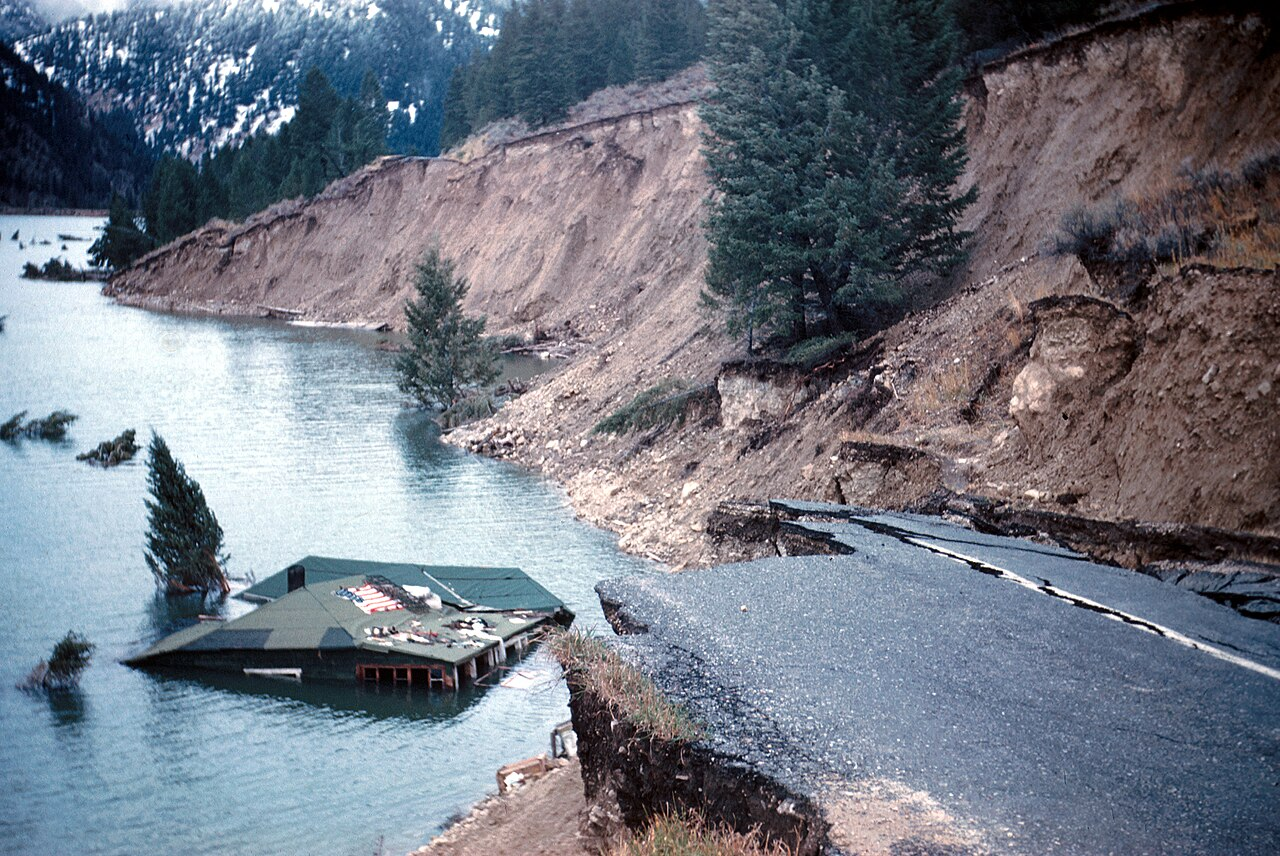
\includegraphics[width=0.6\linewidth]{images/book1/g7-hebgen-road.jpg}

{\small Después del \omterm{def:g4:volcanoes-earthquakes-first-look:earthquake}{terremoto} de Hebgen Lake, en Montana (Estados Unidos),
en agosto de 1959: la carretera que bordeaba el \omterm{def:g1:landscapes-around-us:water}{lago} se hundió en el agua,
y un albergue quedó casi sumergido. Daños como estos son la marca de una
\omterm{def:g7:earthquakes:intensity}{intensidad} alta. Fotografía: I.~J. Witkind, U.S. Geological Survey
(dominio público, vía Wikimedia Commons).}
% ledger: commons:hebgen-road, usgs:mmi
\label{fig:g7:earthquakes:hebgen}
\end{omfigure}

\section{Los tsunamis}

\begin{definition}[Tsunami]\label{def:g7:earthquakes:tsunami}
Un \emph{tsunami}\index{tsunami} es una serie de olas marinas provocadas
por un movimiento brusco del fondo del \omterm{def:g2:water-on-earth:ocean}{mar} --- normalmente un \omterm{def:g4:volcanoes-earthquakes-first-look:earthquake}{terremoto}
submarino, a veces una \omterm{def:g4:volcanoes-earthquakes-first-look:eruption}{erupción} --- que pueden cruzar \omterm{def:g2:water-on-earth:ocean}{océanos} enteros e
inundar las \omterm{def:g1:landscapes-around-us:water}{costas}.
\end{definition}

Cuando una \omterm{def:g7:earthquakes:fault}{falla} submarina se rompe, el fondo del \omterm{def:g2:water-on-earth:ocean}{mar} sube o baja de
golpe y levanta o hace bajar toda la columna de agua que tiene encima. El
agua se propaga en forma de olas. En alta \omterm{def:g2:water-on-earth:ocean}{mar}, un \omterm{def:g7:earthquakes:tsunami}{tsunami} sorprende: rara
vez mide más de un metro de altura, y los barcos ni siquiera notan que
pasa por debajo. Pero es rápido: más de \qty{800}{km/h}, tan rápido como
un avión a reacción. Al llegar a las aguas poco profundas cerca de la
\omterm{def:g1:landscapes-around-us:water}{costa}, frena hasta 30 o \qty{50}{km/h} --- aún más deprisa de lo que nadie
puede correr --- y crece en altura. La mayoría de los \omterm{def:g7:earthquakes:tsunami}{tsunamis} miden menos
de \qty{3}{m} de altura en la \omterm{def:g1:landscapes-around-us:water}{costa}; los mayores superan los \qty{30}{m}.
La primera ola no siempre es la mayor, y las olas pueden seguir llegando
durante horas.
% ledger: nws:tsunami-speed, nws:tsunami-safety

\begin{omfigure}
\begin{tikzpicture}[font=\small, x=1cm, y=1cm]
  % sea floor profile: deep ocean on the left, shelf and coast on the right
  \fill[omSea!35] (0,0) -- (13.2,0) -- (13.2,-0.2) -- (11.4,-0.45) -- (10.2,-1.0) -- (8.8,-2.6) -- (0,-2.6) -- cycle;
  \fill[brown!35] (0,-2.6) -- (8.8,-2.6) -- (10.2,-1.0) -- (11.4,-0.45) -- (13.2,-0.2) -- (13.2,0.5) -- (14.2,1.0) -- (14.2,-3.3) -- (0,-3.3) -- cycle;
  % the broken fault under the sea, at left; one block lifted
  \draw[very thick, red!70!black] (1.9,-3.3) -- (2.3,-2.6);
  \draw[-{Stealth[length=2mm]}, thick] (2.75,-3.1) -- (2.75,-2.75);
  \node[anchor=north west, font=\footnotesize, red!70!black] at (0.1,-3.35) {la falla se rompe, el fondo del mar da un salto};
  % wave: low and long in the deep ocean, short and tall near the coast
  \draw[blue!70!black, thick] (0,0) .. controls (1.2,0.18) and (2.2,0.18) .. (3.4,0)
     -- (5.0,0) .. controls (5.8,0.12) and (6.6,0.12) .. (7.4,0) -- (10.6,0)
     .. controls (11.0,0.55) and (11.6,0.9) .. (12.1,0) -- (13.2,0);
  \node[align=center, font=\footnotesize] at (2.0,0.85) {alta mar: alrededor de 1 m de altura,\\más de 800 km/h};
  \node[align=center, font=\footnotesize] at (11.1,1.55) {cerca de la costa: más lenta\\(30 a 50 km/h), mucho más alta};
  \draw[-{Stealth[length=2.5mm]}, thick, blue!70!black] (4.4,0.45) -- (6.4,0.45);
  \node[font=\footnotesize] at (6.0,-1.5) {miles de metros de profundidad};
  \node[font=\footnotesize] at (12.0,-0.75) {poco profunda};
\end{tikzpicture}

{\small Un \omterm{def:g7:earthquakes:tsunami}{tsunami} cruzando el \omterm{def:g2:water-on-earth:ocean}{océano} (un dibujo, no a escala: la altura de
la ola está muy exagerada). Es baja y muy rápida sobre el \omterm{def:g2:water-on-earth:ocean}{océano} profundo;
frena y crece en las aguas poco profundas cerca de la \omterm{def:g1:landscapes-around-us:water}{costa}.}
% ledger: nws:tsunami-speed
\label{fig:g7:earthquakes:tsunami}
\end{omfigure}

\begin{example}[De Sumatra a Sri Lanka]\label{ex:g7:earthquakes:colombo}
Colombo, la mayor ciudad de Sri Lanka, está a unos \qty{1830}{km} del
\omterm{def:g7:earthquakes:focus}{epicentro} del \omterm{def:g4:volcanoes-earthquakes-first-look:earthquake}{terremoto} de 2004. A \qty{800}{km/h}, un \omterm{def:g7:earthquakes:tsunami}{tsunami} recorre
esa distancia en $1830 \div 800 \approx 2.3$~horas, es decir, unas
2~horas y 17~minutos. Nadie en Sri Lanka sintió el \omterm{def:g4:volcanoes-earthquakes-first-look:earthquake}{terremoto}: la ola llegó
sin más aviso que el propio \omterm{def:g2:water-on-earth:ocean}{mar}.
% ledger: nws:tsunami-speed, usgs:largest (distance and time in figdata/grade-7/quake_counts.py, part tsunami)
\end{example}

\begin{remark}[El aviso que da el mar]\label{rem:g7:earthquakes:natural-warning}
% ledger: nws:tsunami-natural-warning, nws:tsunami-speed, shakeout:dch
En una \omterm{def:g1:landscapes-around-us:water}{costa}, tres señales pueden anunciar un \omterm{def:g7:earthquakes:tsunami}{tsunami}: un \omterm{def:g4:volcanoes-earthquakes-first-look:earthquake}{terremoto} fuerte
o largo; un comportamiento extraño del \omterm{def:g2:water-on-earth:ocean}{mar} --- una \omterm{def:g5:water-shapes-the-land:flood}{inundación} repentina, o
el agua que se retira lejos de la orilla y deja ver el fondo como en una
marea muy baja ---; o un fuerte estruendo que llega del \omterm{def:g2:water-on-earth:ocean}{océano}. Durante la
sacudida, protégete como aprendiste (agáchate, cúbrete, agárrate). Después,
no esperes un aviso oficial: sube lo más alto, o aléjate tierra adentro lo
más lejos que puedas, enseguida. Un \omterm{def:g7:earthquakes:tsunami}{tsunami} causado por un \omterm{def:g4:volcanoes-earthquakes-first-look:earthquake}{terremoto}
cercano puede llegar en pocos minutos.
\end{remark}


\section{Ejercicios}

\begin{exercise}[$\star$]\label{exo:g7:earthquakes:1}
Une cada palabra con su significado: \omterm{def:g7:earthquakes:fault}{falla}; \omterm{def:g7:earthquakes:focus}{hipocentro}; \omterm{def:g7:earthquakes:focus}{epicentro};
\omterm{def:g7:earthquakes:seismometer}{sismómetro}; \omterm{def:g7:earthquakes:magnitude}{magnitud}; \omterm{def:g7:earthquakes:intensity}{intensidad}. (a) El lugar del subsuelo donde empieza
el deslizamiento. (b) Con qué fuerza tembló el suelo en un lugar. (c) Una
rotura de las \omterm{def:g3:stones-pebbles-sand:rock}{rocas} a lo largo de la cual los dos lados se han desplazado.
(d) El punto de la superficie situado encima del \omterm{def:g7:earthquakes:focus}{hipocentro}. (e) El tamaño
de un \omterm{def:g4:volcanoes-earthquakes-first-look:earthquake}{terremoto}, un solo número para cada \omterm{def:g4:volcanoes-earthquakes-first-look:earthquake}{terremoto}. (f) Un instrumento que
registra las sacudidas del suelo.
\end{exercise}

\begin{exercise}[$\star$]\label{exo:g7:earthquakes:2}
El \omterm{def:g7:earthquakes:focus}{hipocentro} de un \omterm{def:g4:volcanoes-earthquakes-first-look:earthquake}{terremoto} está \qty{30}{km} justo por debajo de un
pueblo. (a) ¿Dónde está el \omterm{def:g7:earthquakes:focus}{epicentro}? (b) ¿A qué distancia del \omterm{def:g7:earthquakes:focus}{hipocentro}
está el pueblo? (c) Un segundo pueblo está a \qty{40}{km} del \omterm{def:g7:earthquakes:focus}{epicentro}.
¿Será su \omterm{def:g7:earthquakes:intensity}{intensidad}, en general, mayor o menor que en el primer pueblo?
¿Por qué?
\end{exercise}

\begin{exercise}[$\star$]\label{exo:g7:earthquakes:3}
¿\omterm{def:g7:earthquakes:magnitude}{Magnitud} o \omterm{def:g7:earthquakes:intensity}{intensidad}? (a) ``El \omterm{def:g4:volcanoes-earthquakes-first-look:earthquake}{terremoto} fue de 6.8''. (b) ``En nuestra
calle se cayeron todos los platos y se rompió una chimenea''. (c) ``Fue de
VI en la ciudad y de IV en los pueblos de las \omterm{def:g1:landscapes-around-us:landform}{colinas}''. (d) ``Liberó
32~veces más energía que el del año pasado''.
\end{exercise}

\begin{exercise}[$\star$]\label{exo:g7:earthquakes:4}
¿Verdadero o falso? Corrige las falsas. (a) Los científicos pueden saber
con una semana de antelación cuándo se producirá un \omterm{def:g4:volcanoes-earthquakes-first-look:earthquake}{terremoto}. (b) En alta
\omterm{def:g2:water-on-earth:ocean}{mar}, un \omterm{def:g7:earthquakes:tsunami}{tsunami} es un enorme muro de agua. (c) Un \omterm{def:g4:volcanoes-earthquakes-first-look:earthquake}{terremoto} tiene una sola
\omterm{def:g7:earthquakes:magnitude}{magnitud}, pero muchas \omterm{def:g7:earthquakes:intensity}{intensidades}. (d) La mayoría de los grandes
\omterm{def:g4:volcanoes-earthquakes-first-look:earthquake}{terremotos} se producen cerca de los \omterm{def:g7:plate-tectonics:plate-boundary}{límites de placas}.
\end{exercise}

\begin{exercise}[$\star\star$]\label{exo:g7:earthquakes:5}
Usa el diagrama de los \omterm{def:g4:volcanoes-earthquakes-first-look:earthquake}{terremotos} al año. (a) ¿Cuántos \omterm{def:g4:volcanoes-earthquakes-first-look:earthquake}{terremotos} de
\omterm{def:g7:earthquakes:magnitude}{magnitud} 6 a 6.9 se producen, más o menos, en un año? ¿Y de \omterm{def:g7:earthquakes:magnitude}{magnitud} 7 a
7.9? (b) ¿Cuántas veces menos son los segundos que los primeros? (c) Suma
las tres barras a partir de 7: ¿cuántos \omterm{def:g4:volcanoes-earthquakes-first-look:earthquake}{terremotos} de \omterm{def:g7:earthquakes:magnitude}{magnitud} 7 o más se
producen, más o menos, en un año? (d) El diagrama indica 0.04 al año para
la \omterm{def:g7:earthquakes:magnitude}{magnitud} 9 o más. ¿Cuántos son en 50~años?
\end{exercise}

\begin{exercise}[$\star\star$]\label{exo:g7:earthquakes:6}
Usa el método para comparar \omterm{def:g7:earthquakes:magnitude}{magnitudes}. (a) ¿Cuántas veces más energía
libera un \omterm{def:g4:volcanoes-earthquakes-first-look:earthquake}{terremoto} de \omterm{def:g7:earthquakes:magnitude}{magnitud} 7 que uno de \omterm{def:g7:earthquakes:magnitude}{magnitud} 6? (b) ¿Y uno de
\omterm{def:g7:earthquakes:magnitude}{magnitud} 8 que uno de \omterm{def:g7:earthquakes:magnitude}{magnitud} 6? (c) Entre la \omterm{def:g7:earthquakes:magnitude}{magnitud} 6 y la 8, ¿cuántas
veces más grandes son sus ondas en el \omterm{def:g7:earthquakes:seismometer}{sismograma}, a la misma distancia?
\end{exercise}

\begin{exercise}[$\star\star$]\label{exo:g7:earthquakes:7}
Usa \qty{8}{km} por cada segundo de retraso entre las ondas más rápidas y
las más lentas. (a) Una estación registra un retraso de \qty{5}{s}. ¿A qué
distancia se produjo el \omterm{def:g4:volcanoes-earthquakes-first-look:earthquake}{terremoto}? (b) Otra registra \qty{25}{s}. (c) Un
\omterm{def:g4:volcanoes-earthquakes-first-look:earthquake}{terremoto} se produjo a \qty{120}{km} de una estación: ¿qué retraso leerá
la estación? (d) ¿Por qué una sola estación no puede decir dónde está el
\omterm{def:g7:earthquakes:focus}{epicentro}?
\end{exercise}

\begin{exercise}[$\star\star$]\label{exo:g7:earthquakes:8}
Usa la tabla de \omterm{def:g7:earthquakes:intensity}{intensidades}. Da la \omterm{def:g7:earthquakes:intensity}{intensidad} de cada testimonio.
(a) ``Lo sintió casi todo el mundo; nos despertamos y se rompieron dos
vasos''. (b) ``Solo lo sintió mi abuela, que descansaba en el piso de
arriba; la lámpara se balanceó''. (c) ``Cayeron muros y chimeneas; varias
casas se derrumbaron en parte''. (d) El mismo \omterm{def:g4:volcanoes-earthquakes-first-look:earthquake}{terremoto} dio los testimonios
(a) y (c). Explica cómo es posible.
\end{exercise}

\begin{exercise}[$\star\star$]\label{exo:g7:earthquakes:9}
De los 7\,031 \omterm{def:g4:volcanoes-earthquakes-first-look:earthquake}{terremotos} de \omterm{def:g7:earthquakes:magnitude}{magnitud}~6 o más de 1976--2025, 5\,561 tuvieron
su \omterm{def:g7:earthquakes:focus}{hipocentro} a menos de \qty{70}{km} de profundidad. (a) ¿Cuántos tuvieron
un \omterm{def:g7:earthquakes:focus}{hipocentro} más profundo? (b) ¿Qué porcentaje es? Redondea al número
entero más cercano. (c) Los profundos se producen donde una \omterm{def:g7:plate-tectonics:plate}{placa} se hunde
bajo otra. Explica por qué allí pueden empezar a tanta profundidad.
\end{exercise}

\begin{exercise}[$\star\star$]\label{exo:g7:earthquakes:10}
Malé, la capital de las Maldivas, está a unos \qty{2500}{km} del
\omterm{def:g7:earthquakes:focus}{epicentro} del \omterm{def:g4:volcanoes-earthquakes-first-look:earthquake}{terremoto} de 2004. (a) A \qty{800}{km/h}, ¿cuánto tardó el
\omterm{def:g7:earthquakes:tsunami}{tsunami} en llegar? Da las horas y los minutos. (b) ¿Cuánto más tarde llegó
que a Colombo (2~horas y 17~minutos)? (c) Con semejantes tiempos, ¿por qué
un sistema de alerta habría podido salvar muchas vidas?
\end{exercise}

\begin{exercise}[$\star\star\star$]\label{exo:g7:earthquakes:11}
Un \omterm{def:g7:earthquakes:tsunami}{tsunami} cruza \qty{400}{km} de \omterm{def:g2:water-on-earth:ocean}{océano} profundo a \qty{800}{km/h} y
después los últimos \qty{20}{km} de aguas poco profundas a
\qty{40}{km/h}. (a) ¿Cuántos minutos tarda en la parte profunda? (b) ¿Y en
la parte poco profunda? (c) ¿Cuánto dura todo el recorrido? (d) ¿Qué
tienen de sorprendente tus respuestas? (e) ¿Por qué crece la ola en altura
a medida que frena?
\end{exercise}

\begin{exercise}[$\star\star\star$]\label{exo:g7:earthquakes:12}
(a) ¿Cuántas veces más energía libera un \omterm{def:g4:volcanoes-earthquakes-first-look:earthquake}{terremoto} de \omterm{def:g7:earthquakes:magnitude}{magnitud} 9 que uno de
\omterm{def:g7:earthquakes:magnitude}{magnitud} 6? (b) Cada año hay unos 127 \omterm{def:g4:volcanoes-earthquakes-first-look:earthquake}{terremotos} de \omterm{def:g7:earthquakes:magnitude}{magnitud} 6 a 6.9.
Supón que cada uno libera la energía de uno de \omterm{def:g7:earthquakes:magnitude}{magnitud} 6. ¿Cuántos años
de esos \omterm{def:g4:volcanoes-earthquakes-first-look:earthquake}{terremotos} hacen falta para liberar la energía de un solo
\omterm{def:g4:volcanoes-earthquakes-first-look:earthquake}{terremoto} de \omterm{def:g7:earthquakes:magnitude}{magnitud}~9? (c) ¿Qué te dice esto sobre la parte de la
energía que se llevan los \omterm{def:g4:volcanoes-earthquakes-first-look:earthquake}{terremotos} más grandes?
\end{exercise}

\section{Problema: ¿dónde tembló el suelo?}

\begin{problem}[{Problema de fin de semana --- tres estaciones registran un
terremoto submarino, se halla el epicentro en el mapa y se avisa a la
ciudad de Port Hale antes de que llegue el tsunami}]
\label{pb:g7:earthquakes:1}
% ledger: nws:tsunami-speed, usgs:seismograph, data:prem (figdata/grade-7/epicentre.py)
Un \omterm{def:g4:volcanoes-earthquakes-first-look:earthquake}{terremoto} se produce bajo el \omterm{def:g2:water-on-earth:ocean}{mar} de una \omterm{def:g1:landscapes-around-us:water}{costa} inventada. Tres
estaciones sismológicas, A, B y C, están en tierra firme; la ciudad de
Port Hale está en una isla (\omterm{def:g2:drawing-to-map:map}{mapa} de abajo; un cuadrado mide \qty{20}{km}).
En esta región, cada segundo de retraso entre las ondas más rápidas y las
más lentas equivale a \qty{8}{km}. Las estaciones registran:

\begin{center}
\small
\begin{tabular}{|c|c|c|}
\hline
\textbf{estación} & \textbf{llegan las ondas más rápidas} & \textbf{llegan las ondas más lentas} \\
\hline
A & 10:15:25 & 10:15:45 \\
B & 10:15:16 & 10:15:29 \\
C & 10:15:19 & 10:15:34 \\
\hline
\end{tabular}
\end{center}

\medskip
\noindent\textbf{Parte I --- Tres estaciones.}\par\nopagebreak
\begin{enumerate}[beginpenalty=10000]
  \item Para cada estación, halla el retraso entre las dos llegadas, en
        segundos.
  \item ¿Qué estación está más cerca del \omterm{def:g4:volcanoes-earthquakes-first-look:earthquake}{terremoto}? ¿Cómo lo sabes sin
        hacer ningún cálculo?
  \item Halla la distancia de cada estación al \omterm{def:g4:volcanoes-earthquakes-first-look:earthquake}{terremoto}.
  \item La distancia de la estación A no basta para decir dónde se produjo
        el \omterm{def:g4:volcanoes-earthquakes-first-look:earthquake}{terremoto}. Describe todos los lugares que están a esa distancia
        de A.
\end{enumerate}

\begin{center}
\begin{tikzpicture}
  \begin{axis}[axis equal image, width=12cm, xmin=-60, xmax=360, ymin=-200, ymax=260,
      xtick={-60,-40,...,360}, ytick={-200,-180,...,260}, xticklabels={}, yticklabels={},
      major tick length=0pt,
      axis background/.style={fill=omSea!25}, clip mode=individual]
    \addplot[fill=omLithAlluv, draw=black!50, line width=0.4pt] table[x=x, y=y] {figdata/out/grade-7-epicentre-p-west.dat};
    \addplot[fill=omLithAlluv, draw=black!50, line width=0.4pt] table[x=x, y=y] {figdata/out/grade-7-epicentre-p-north.dat};
    \addplot[fill=omLithAlluv, draw=black!50, line width=0.4pt] table[x=x, y=y] {figdata/out/grade-7-epicentre-p-island.dat};
    % the grid over land and sea, drawn before the labels
    \pgfplotsinvokeforeach{-40,-20,0,20,40,60,80,100,120,140,160,180,200,220,240,260,280,300,320,340}{\draw[black!15] (axis cs:#1,-200) -- (axis cs:#1,260);}
    \pgfplotsinvokeforeach{-180,-160,-140,-120,-100,-80,-60,-40,-20,0,20,40,60,80,100,120,140,160,180,200,220,240}{\draw[black!15] (axis cs:-60,#1) -- (axis cs:360,#1);}
    \addplot[only marks, mark=triangle*, mark size=3.2pt, black,
        nodes near coords, point meta=explicit symbolic,
        nodes near coords style={font=\small\bfseries, anchor=south west}]
      table[x=x, y=y, meta=name] {figdata/out/grade-7-epicentre-p-stations.dat};
    \addplot[only marks, mark=square*, mark size=2.4pt, red!70!black,
        nodes near coords, point meta=explicit symbolic,
        nodes near coords style={font=\small, anchor=north east, fill=omSea!25, inner sep=1pt}]
      table[x=x, y=y, meta=name] {figdata/out/grade-7-epicentre-p-town.dat};
    \draw[-{Stealth[length=2.5mm]}, line width=0.8pt] (axis cs:330,200) -- (axis cs:330,245);
    \node[font=\scriptsize\bfseries, anchor=north] at (axis cs:330,200) {N};
    \node[font=\scriptsize, anchor=west, fill=omLithAlluv, inner sep=1pt] at (axis cs:170,240) {1 cuadrado = 20 km};
    \fill (axis cs:-60,-200) circle (1.5pt);
    \node[font=\small\bfseries, anchor=north east] at (axis cs:-60,-200) {O};
  \end{axis}
\end{tikzpicture}
\end{center}
% ledger: (invented map: figdata/grade-7/epicentre.py, parts p-west, p-north, p-island, p-stations, p-town)

\medskip
\noindent\textbf{Parte II --- Hallar el epicentro.}\par\nopagebreak
\begin{enumerate}[resume, beginpenalty=10000]
  \item Un cuadrado mide \qty{20}{km}. ¿Cuántos cuadrados mide el radio de
        cada círculo?
  \item Coloca la esquina O abajo a la izquierda del \omterm{def:g2:drawing-to-map:map}{mapa}. La estación C
        está 3~cuadrados al este y 14.5~cuadrados al norte de O; si avanzas
        6~cuadrados (\qty{120}{km}) hacia el este desde C, llegas a un
        punto~E. Comprueba en el \omterm{def:g2:drawing-to-map:map}{mapa} que E también está en los círculos de
        A y de B: es el \omterm{def:g7:earthquakes:focus}{epicentro}. ¿A cuántos cuadrados al este y al norte
        de O está?
  \item ¿Está el \omterm{def:g7:earthquakes:focus}{epicentro} en tierra firme o bajo el \omterm{def:g2:water-on-earth:ocean}{mar}? ¿Por qué importa?
  \item La \omterm{def:g7:earthquakes:magnitude}{magnitud} fue de 7.4. ¿Cuántas veces más energía que un \omterm{def:g4:volcanoes-earthquakes-first-look:earthquake}{terremoto}
        de \omterm{def:g7:earthquakes:magnitude}{magnitud}~6.4 liberó?
\end{enumerate}

\medskip
\noindent\textbf{Parte III --- La ola llega a la costa.}\par\nopagebreak
\begin{enumerate}[resume, beginpenalty=10000]
  \item En el \omterm{def:g2:drawing-to-map:map}{mapa}, Port Hale está a 12~cuadrados del \omterm{def:g7:earthquakes:focus}{epicentro}. ¿Cuántos
        kilómetros son?
  \item A \qty{800}{km/h}, ¿cuántos minutos tarda el \omterm{def:g7:earthquakes:tsunami}{tsunami} en llegar a
        Port Hale?
  \item Localizar el \omterm{def:g4:volcanoes-earthquakes-first-look:earthquake}{terremoto} y enviar el aviso lleva 5~minutos desde que
        empieza la sacudida. ¿Cuánto tiempo después del \omterm{def:g4:volcanoes-earthquakes-first-look:earthquake}{terremoto} llega el
        aviso a Port Hale?
  \item ¿Cuántos minutos tienen los habitantes de Port Hale para llegar a
        un lugar alto antes de que llegue el \omterm{def:g7:earthquakes:tsunami}{tsunami}?
\end{enumerate}
\end{problem}
